% GENERATED by make_paper_assets.py -- do not edit by hand.
\begin{figure*}[t]
\centering
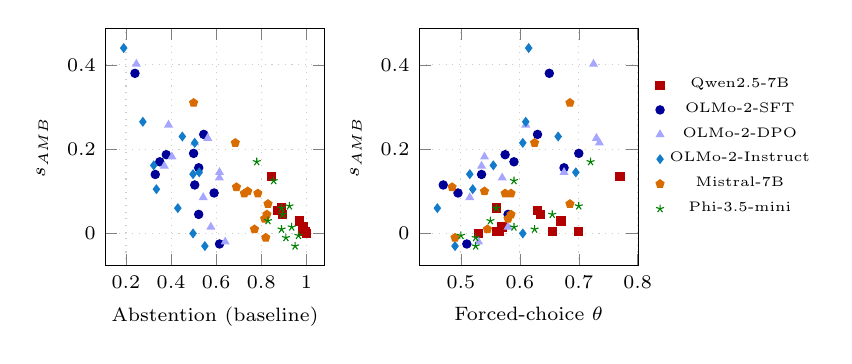
\begin{tikzpicture}
\begin{axis}[name=a, width=0.36\textwidth, height=4.6cm,
  xlabel={Abstention (baseline)}, ylabel={$s_{\text{AMB}}$},
  tick label style={font=\scriptsize}, label style={font=\scriptsize}, grid=major, grid style={dotted, gray!40}]
\addplot[only marks, mark=square*, mark size=1.5pt, red!70!black] coordinates {(0.8450,0.1350) (0.8950,0.0450) (0.9850,0.0150) (0.8750,0.0550) (0.9700,0.0300) (0.9950,0.0050) (0.9950,0.0050) (1.0000,0.0000) (0.8900,0.0600) (0.9950,0.0050) (0.9850,0.0050)};
\addplot[only marks, mark=*, mark size=1.5pt, blue!60!black] coordinates {(0.2400,0.3800) (0.3300,0.1400) (0.3500,0.1700) (0.3788,0.1869) (0.5450,0.2350) (0.5226,0.0452) (0.5909,0.0960) (0.5050,0.1150) (0.5226,0.1558) (0.5000,0.1900) (0.6150,-0.0250)};
\addplot[only marks, mark=triangle*, mark size=1.5pt, blue!35!white] coordinates {(0.2462,0.4020) (0.3700,0.1600) (0.3889,0.2576) (0.4040,0.1818) (0.5628,0.2261) (0.5765,0.0153) (0.6142,0.1320) (0.5427,0.0854) (0.6150,0.1450) (0.5050,0.2150) (0.6400,-0.0200)};
\addplot[only marks, mark=diamond*, mark size=1.5pt, cyan!60!blue] coordinates {(0.1900,0.4400) (0.3350,0.1050) (0.2750,0.2650) (0.3232,0.1616) (0.5050,0.2150) (0.4975,0.0000) (0.4975,0.1407) (0.4300,0.0600) (0.5250,0.1450) (0.4500,0.2300) (0.5500,-0.0300)};
\addplot[only marks, mark=pentagon*, mark size=1.5pt, orange!85!black] coordinates {(0.5000,0.3100) (0.6900,0.1100) (0.7250,0.0950) (0.7400,0.1000) (0.7850,0.0950) (0.7700,0.0100) (0.8150,0.0350) (0.8200,-0.0100) (0.8300,0.0700) (0.6850,0.2150) (0.8250,0.0450)};
\addplot[only marks, mark=star, mark size=1.5pt, green!50!black] coordinates {(0.7800,0.1700) (0.8300,0.0300) (0.8950,0.0450) (0.8900,0.0100) (0.8550,0.1250) (0.9095,-0.0101) (0.9350,0.0150) (0.9650,-0.0050) (0.8900,0.0600) (0.9250,0.0650) (0.9500,-0.0300)};
\end{axis}
\begin{axis}[at={(a.east)}, xshift=1.2cm, anchor=west, width=0.36\textwidth, height=4.6cm,
  xlabel={Forced-choice $\theta$}, ylabel={$s_{\text{AMB}}$},
  tick label style={font=\scriptsize}, label style={font=\scriptsize}, grid=major, grid style={dotted, gray!40},
  legend style={at={(1.04,0.5)}, anchor=west, font=\tiny, draw=none}]
\addplot[only marks, mark=square*, mark size=1.5pt, red!70!black] coordinates {(0.7700,0.1350) (0.6350,0.0450) (0.5700,0.0150) (0.6300,0.0550) (0.6700,0.0300) (0.5600,0.0050) (0.6550,0.0050) (0.5300,0.0000) (0.5600,0.0600) (0.7000,0.0050) (0.5650,0.0050)};\addlegendentry{Qwen2.5-7B}
\addplot[only marks, mark=*, mark size=1.5pt, blue!60!black] coordinates {(0.6500,0.3800) (0.5350,0.1400) (0.5900,0.1700) (0.5750,0.1869) (0.6300,0.2350) (0.5800,0.0452) (0.4950,0.0960) (0.4700,0.1150) (0.6750,0.1558) (0.7000,0.1900) (0.5100,-0.0250)};\addlegendentry{OLMo-2-SFT}
\addplot[only marks, mark=triangle*, mark size=1.5pt, blue!35!white] coordinates {(0.7250,0.4020) (0.5350,0.1600) (0.6100,0.2576) (0.5400,0.1818) (0.7300,0.2261) (0.5800,0.0153) (0.5700,0.1320) (0.5150,0.0854) (0.6750,0.1450) (0.7350,0.2150) (0.5300,-0.0200)};\addlegendentry{OLMo-2-DPO}
\addplot[only marks, mark=diamond*, mark size=1.5pt, cyan!60!blue] coordinates {(0.6150,0.4400) (0.5200,0.1050) (0.6100,0.2650) (0.5550,0.1616) (0.6050,0.2150) (0.6050,0.0000) (0.5150,0.1407) (0.4600,0.0600) (0.6950,0.1450) (0.6650,0.2300) (0.4900,-0.0300)};\addlegendentry{OLMo-2-Instruct}
\addplot[only marks, mark=pentagon*, mark size=1.5pt, orange!85!black] coordinates {(0.6850,0.3100) (0.4850,0.1100) (0.5850,0.0950) (0.5400,0.1000) (0.5750,0.0950) (0.5450,0.0100) (0.5800,0.0350) (0.4900,-0.0100) (0.6850,0.0700) (0.6250,0.2150) (0.5850,0.0450)};\addlegendentry{Mistral-7B}
\addplot[only marks, mark=star, mark size=1.5pt, green!50!black] coordinates {(0.7200,0.1700) (0.5500,0.0300) (0.6550,0.0450) (0.6250,0.0100) (0.5900,0.1250) (0.5250,-0.0101) (0.5900,0.0150) (0.5000,-0.0050) (0.5600,0.0600) (0.7000,0.0650) (0.5250,-0.0300)};\addlegendentry{Phi-3.5-mini}
\end{axis}
\end{tikzpicture}
\caption{The 66 (checkpoint $\times$ category) cells behind Figure~\ref{fig:variance}.
Left: the reported score falls with abstention. Right: it rises with the
stereotype-aligned rate $\theta$. Both relationships hold at once, which is why
neither alone summarises the score.}
\label{fig:cells}
\end{figure*}
